% ---------------------------------------------------------------------------- %
%                                  !! TODO  !!
%
% Create version for non-CMU that covers more and has better flow:
% - Add TerraFlow algorithm
% - Change Time-forward Processing to be solving the exact same problem.
% ---------------------------------------------------------------------------- %

\documentclass[english, aspectratio=169]{beamer}

% ---------------------------------------------------------------------------- %
% Load base preamble
% ---------------------------------------------------------------------------- %
\usepackage{import}
\subimport{./preamble/}{beamer.tex}

\usepackage{tipa}
\usepackage{mathdots}
\usepackage[normalem]{ulem}

\metroset{sectionpage=none}

% ---------------------------------------------------------------------------- %
% Local macros
% ---------------------------------------------------------------------------- %

% types
\newcommand{\B}[0]{\ensuremath{\mathbb{B}}}

% I/O efficient
\newcommand{\scan}[0]{\text{scan}}
\newcommand{\sort}[0]{\text{sort}}

% Adiar
\newcommand{\triple}[3]{\ensuremath{(#1, #2, #3)}}
\renewcommand{\arc}[3]{\ensuremath{#1 \xrightarrow{_{#2}} #3}}

% Tikz plots
\tikzstyle{plot_cache_1}=[color=red, mark=none, line width=1pt]
\tikzstyle{plot_cache_500}=[color=purple, mark=none, line width=1pt]
\tikzstyle{plot_cache_1000}=[color=blue, mark=none, line width=1pt]

\tikzstyle{plot_adiar}=[color=red, mark=o, mark size=1pt, line width=0.9pt]
\tikzstyle{plot_other}=[color=blue, mark=diamond, mark size=1pt, line width=0.9pt]

% Horizontal legends: https://tex.stackexchange.com/a/101578
% argument #1: any options
\makeatletter
\newenvironment{customlegend}[1][]{%
  \begingroup
  % inits/clears the lists (which might be populated from previous
  % axes):
  \pgfplots@init@cleared@structures
  \pgfplotsset{#1}%
}{%
  % draws the legend:
  \pgfplots@createlegend
  \endgroup
}%

% makes \addlegendimage available (typically only available within an
% axis environment):
\def\addlegendimage{\pgfplots@addlegendimage}
\makeatother

% ---------------------------------------------------------------------------- %
% TITLEPAGE
% ---------------------------------------------------------------------------- %
\title{I/O-Efficient Algorithms and Data Structures}

\author{\textbf{Steffan Christ S\o lvsten}}

\date{$9^{\text{th}}$ of September, 2023}

\institute{
\includegraphics[width=0.2\linewidth]{./external/aulogo_uk_var2_black.eps}}

% ---------------------------------------------------------------------------- %
% Content
% ---------------------------------------------------------------------------- %
\begin{document}

\titleframe

\section{I/O-model}

\begin{frame}
    \begin{figure}
    \centering

    \LARGE

    \begin{tikzpicture}[scale=1.5]
      \node at (0.50,0) (i1) {$0$,};
      \node at (1.00,0)      {$1$,};
      \node at (1.50,0)      {$2$,};
      \node at (2.20,0) (d1) {$\cdots$};
      \node at (3.00,0) (i2) {$i$,};
      \node at (3.75,0)      {$i+1$,};
      \node at (4.70,0) (d2) {$\cdots$};
      \node at (5.40,0) (i3) {$2i$,};
      \node at (6.30,0)      {$2i+1$,};
      \node at (7.30,0) (d3) {$\cdots$};
      \node at (7.85,0) (d4) {$\cdots$};
      \node at (9.00,0)      {$N-1$};

      \onslide<2->{
        \draw[->, thick, densely dashed] (i1) edge[bend left=70] (i2);
      }

      \onslide<3->{
        \draw[->, thick, densely dashed] (i2) edge[bend left=70] (i3);
      }

      \onslide<4->{
        \draw[->, thick, densely dashed] (i3) edge[bend left=70] (d4);
      }

      \onslide<5->{
        \draw[->, thick, densely dashed] (d4) edge[bend left=90] (d1);
        \draw[->, thick, densely dashed, gray]
          (d1) edge[bend left=70] (d2)
          (d2) edge[bend left=70] (d3)
        ;
      }
    \end{tikzpicture}
  \end{figure}

\end{frame}

\begin{frame}
  \begin{figure}
    \centering

    \begin{tikzpicture}
      \begin{axis}[%
        width=0.90\linewidth, height=0.42\linewidth,
        every tick label/.append style={font=\scriptsize},
        % x-axis
        xlabel={Vector size ($N$)},
        xmajorgrids=true,
        xmin=-1900000,
        xmax=18000000,
        % y-axis
        ymin=100,
        ymax=700,
        %ytick distance={0.5},
        ylabel={Time (ms)},
        yminorgrids=true,
        ymajorgrids=true,
        grid style={dashed,black!20},
        ]

        \only<3-> {
          \addplot+ [style=plot_cache_1000]
          table {./data/cache_crusher_i=1000.tex};
        }
        %\only<3-> {
        %  \addplot+ [style=plot_cache_500]
        %  table {./data/cache_crusher_i=500.tex};
        %}
        \only<2-> {
          \addplot+ [style=plot_cache_1]
          table {./data/cache_crusher_i=1.tex};
        }
      \end{axis}

    \end{tikzpicture}

    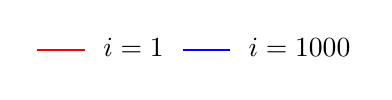
\begin{tikzpicture}
      \begin{customlegend}[
        legend columns=-1,
        legend style={draw=none,column sep=1ex},
        legend entries={
          $i=1$,
%          $i=500$,
          $i=1000$
        }
        ]
        \addlegendimage{style=plot_cache_1}
%        \addlegendimage{style=plot_cache_500}
        \addlegendimage{style=plot_cache_1000}
      \end{customlegend}
    \end{tikzpicture}

  \end{figure}
\end{frame}

\blankframe

\begin{frame}
  % Numbers from:
% - Intel® 64 and IA-32 Architectures Optimization Reference Manual
%   + Cache: Table 2-7/2-14
%   + RAM:   3.6.10 Locality Enhancement
% - www.lighterra.com/papers/modernmicroprocessors/
%   + SSD: Extrapolation from the 2.000.000 to fit Intel's Manual.
% - imada.sdu.dk/u/rolf/Edu/DM79/E04/Slides/IOModel.pdf
%   + HDD: Extrapolation from the 2.000.000 to fit Intel's Manual.

\begin{center}
  \begin{tikzpicture}
    % ALU
    \node[draw, trapezium, shape border rotate=180, text width=0.8cm, align=center] at (0,0) (cpu) {CPU};

    % Cache
    \draw[draw=gray, rounded corners=3pt, densely dotted, line width = 0.6pt]
    (-1.3,2.3) rectangle ++(2.6,-1.6);

    \node[ draw, rectangle, text width=0.3cm, align=center] at (0,1)    (l1) {\tiny L1};
    \node[ draw, rectangle, text width=0.8cm, align=center] at (0,1.45) (l2) {\tiny L2};
    \node[ draw, rectangle, text width=2cm, align=center]   at (0,1.95) (l3) {\footnotesize L3};

    \path[->]
    (cpu) edge[bend left=25] (l1)
    (l1) edge[bend left=25] (cpu) ;
    \onslide<2->{\node at (2.8,0.5) {$\sim$ 4 -- 50 CPU Cycles};}

    % Main memory
    \node[draw, rectangle, text width=4cm, align=center] at (0,3.5) (ram) {RAM};

    \path[->]
      (l3) edge[bend left=40] (ram)
      (ram) edge[bend left=40] (l3)
    ;
    \onslide<2->{
      \node at (2.6,2.7) {$\sim$ 200 CPU Cycles};
    }

    % Disk
    \only<-2> { \node[ draw, cylinder, minimum width=8cm, aspect=0.3,
      align=center, shape border rotate=90 ] at (0,5.5) (disk) {SSD};
    }
    \onslide<3> { \node[ draw, cylinder, minimum width=12cm, aspect=0.26,
      align=center, shape border rotate=90 ] at (0,5.5) (disk) {HDD};
    }

    \path[->]
      (disk) edge[bend left=40] (ram)
      (ram) edge[bend left=40] (disk)
    ;
    \only<2>{
      \node at (3,4.5) {$\sim$ 200.000+ CPU Cycles};
    }
    \onslide<3->{
      \node at (3.25,4.5) {$\sim$ 20.000.000+ CPU Cycles};
    }
  \end{tikzpicture}
\end{center}
\end{frame}

\begin{frame}
  \frametitle{I/O Model\\Aggarwal and Vitter '87}

  \begin{figure}
    \centering
    % TODO: Colour internal memory?
    \begin{tikzpicture}
  % ALU
  \node[
  draw,
  trapezium,
  shape border rotate=180,
  text width=1cm,
  align=center,
  ] at (0.03,0) (cpu) {CPU};

  % Main memory
  \begin{scope}
    \clip(-1.13,1) rectangle (1.19,1.4);
    \filldraw[
    color=black!60!white,
    fill=black!5!white,
    pattern=vertical lines,
    pattern color=black!30!white
    ] (-9,1.25) rectangle ++(18,0.5)
    ;
  \end{scope}

  \node[
  draw,
  rectangle,
  text width=2.08cm,
  align=center,
  ] at (0.03,1.5) (m) {$M$};

  % Disk
  \begin{scope}
    \clip(-6,2.5) rectangle (6,2.9);
    \filldraw[
    color=black!60!white,
    fill=black!5!white,
    pattern=vertical lines,
    pattern color=black!30!white
    ] (-9,2.75) rectangle ++(18,0.5)
    ;
  \end{scope}

  \node[
  draw,
  rectangle,
  text width=5.04cm,
  align=center,
  ] at (0.03,3) (n) {$N$};

  \path[->]
  (cpu) edge[bend left=40] (m)
  (m) edge[bend left=40] (cpu)

  (n) edge[bend left=40] (m)
  (m) edge[bend left=40] (n)
  ;

  \node at (0.02,2.24) {\textcolor{gray}{$B$}};
\end{tikzpicture}

  \end{figure}
\end{frame}

\section{Files and Sorting}

\begin{frame}
  \frametitle{I/O Model : Sequential Access\\Aggarwal and Vitter '87}

    \begin{figure}
    \centering

    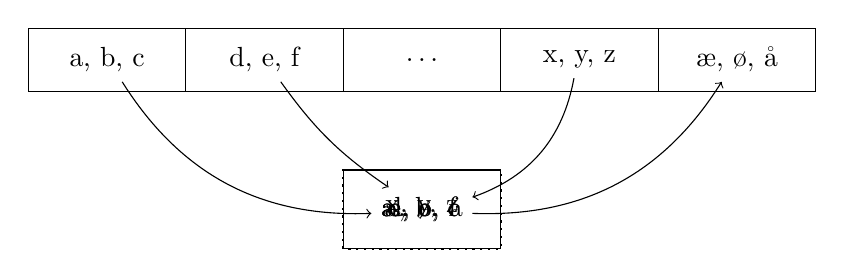
\begin{tikzpicture}
      % Block 1
      \draw[] (0,0)  rectangle ++(2,0.8) node[pos=.5] (b1) {a, b, c};

      % Block 2
      \draw[] (2,0)  rectangle ++(2,0.8) node[pos=.5] (b2) {d, e, f};

      % Block 3
      \draw[] (4,0)  rectangle ++(2,0.8) node[pos=.5] {$\dots$};

      % Block 4
      \draw[] (6,0)  rectangle ++(2,0.8) node[pos=.5] (b3) {x, y, z};

      % Block 5
      \onslide<10-> {
        \draw[] (8,0) rectangle ++(2,0.8) node[pos=.5] (b4) {\ae, \o, \aa};
      }

      % Memory
      \draw[dotted, thick] (4,-2) rectangle ++(2,1) node[pos=.5] (M) {};

      % NOTE: Tikz does not like \only<>/\onslide<> within a node's text (even
      % if the output seems correct. So to not get compiler errors it must be
      % copy-pasted...
      %
      % On the bright side, it also gives a very cool "active block" effect.
      \onslide<2> {
        \draw[] (4,-2) rectangle ++(2,1) node[pos=.5] (M) {a, b, c};
      }
      \onslide<3> {
        \draw[] (4,-2) rectangle ++(2,1) node[pos=.5] (M) {d, e, f};
      }
      \onslide<5> {
        \draw[] (4,-2) rectangle ++(2,1) node[pos=.5] (M) {x, y, z};
      }
      \onslide<7> {
        \draw[] (4,-2) rectangle ++(2,1) node[pos=.5] (M) {\ae\phantom{, \o, \aa}};
      }
      \onslide<8> {
        \draw[] (4,-2) rectangle ++(2,1) node[pos=.5] (M) {\ae, \o\phantom{, \aa}};
      }
      \onslide<9> {
        \draw[] (4,-2) rectangle ++(2,1) node[pos=.5] (M) {\ae, \o, \aa};
      }

      % Arrows
      \onslide<2>  { \draw[->] (b1) edge[bend right]    (M); }
      \onslide<3>  { \draw[->] (b2) edge[bend right=10] (M); }
      \onslide<5>  { \draw[->] (b3) edge[bend left]     (M); }
      \onslide<10> { \draw[->] (M)  edge[bend right]    (b4); }
    \end{tikzpicture}
  \end{figure}


  \onslide<11-> {
    \begin{table}
      \begin{tabular}{rcl}
        Time   & : & $N$
        \\
        I/O    & : & $N/B$
        \\
        Memory & : & $B$
      \end{tabular}
    \end{table}
  }
\end{frame}

\begin{frame}
  \frametitle{I/O Model : Stack\\\phantom{Aggarwal and Vitter '87}}

    \begin{figure}
    \centering

    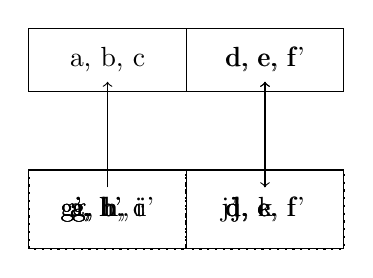
\begin{tikzpicture}
      \onslide<8-> {
        % Block 1
        \draw[] (0,0)  rectangle ++(2,0.8) node[pos=.5] (b1) {a, b, c};
      }

      \onslide<12-25> {
        % Block 2
        \draw[] (2,0)  rectangle ++(2,0.8) node[pos=.5] (b2) {d, e, f\phantom{'}};
      }
      \onslide<26-> {
        % Block 2
        \draw[] (2,0)  rectangle ++(2,0.8) node[pos=.5] (b2) {d, e, f'};
      }

      % NOTE: Tikz does not like \only<>/\onslide<> within a node's text (even
      % if the output seems correct. So to not get compiler errors it must be
      % copy-pasted...

      % Memory 1
      \draw[dotted, thick] (0,-2) rectangle ++(2,1) node[pos=.5] (M1) {};

      \onslide<2> {
        \draw[] (0,-2) rectangle ++(2,1) node[pos=.5] (M1) {a\phantom{, b, c}};
      }
      \onslide<3> {
        \draw[] (0,-2) rectangle ++(2,1) node[pos=.5] (M1) {a, b\phantom{, c}};
      }
      \onslide<4-7> {
        \draw[] (0,-2) rectangle ++(2,1) node[pos=.5] (M1) {a, b, c};
      }

      \onslide<9,18> {
        \draw[] (0,-2) rectangle ++(2,1) node[pos=.5] (M1) {g\phantom{, h, i}};
      }
      \onslide<10,17> {
        \draw[] (0,-2) rectangle ++(2,1) node[pos=.5] (M1) {g, h\phantom{, i}};
      }
      \onslide<11-16> {
        \draw[] (0,-2) rectangle ++(2,1) node[pos=.5] (M1) {g, h, i};
      }

      \onslide<23> {
        \draw[] (0,-2) rectangle ++(2,1) node[pos=.5] (M1) {g'\phantom{, h', i'}};
      }
      \onslide<24> {
        \draw[] (0,-2) rectangle ++(2,1) node[pos=.5] (M1) {g', h'\phantom{, i'}};
      }
      \onslide<25-> {
        \draw[] (0,-2) rectangle ++(2,1) node[pos=.5] (M1) {g', h', i'};
      }

      % Memory 2
      \draw[dotted, thick] (2,-2) rectangle ++(2,1) node[pos=.5] (M2) {};

      \onslide<5> {
        \draw[] (2,-2) rectangle ++(2,1) node[pos=.5] (M2) {d\phantom{, e, f'}};%
      }
      \onslide<6,21> {
        \draw[] (2,-2) rectangle ++(2,1) node[pos=.5] (M2) {d, e\phantom{, f'}};%
      }
      \onslide<7-11,20> {
        \draw[] (2,-2) rectangle ++(2,1) node[pos=.5] (M2) {d, e, f\phantom{'}};%
      }
      \onslide<22-25> {
        \draw[] (2,-2) rectangle ++(2,1) node[pos=.5] (M2) {d, e, f'};%
      }
      \onslide<27-> {
        \draw[] (2,-2) rectangle ++(2,1) node[pos=.5] (M2) {j'\phantom{, k', l'}};%
      }

      \onslide<13, 15> {
        \draw[] (2,-2) rectangle ++(2,1) node[pos=.5] (M2) {j\phantom{, k, l}};
      }
      \onslide<14> {
        \draw[] (2,-2) rectangle ++(2,1) node[pos=.5] (M2) {j, k\phantom{, l}};
      }

      % Arrows
      \onslide<8>  { \draw[->] (M1) edge (b1); }
      \onslide<12> { \draw[->] (M2) edge (b2); }
      \onslide<20> { \draw[->] (b2) edge (M2); }
      \onslide<26> { \draw[->] (M2) edge (b2); }
    \end{tikzpicture}
  \end{figure}


  \onslide<25-> {
    \begin{table}
      \begin{tabular}{rcl}
        Time   & : & $O(N)$
        \\
        I/O    & : & $O(N/B)$
        \\
        Memory & : & $2B$
      \end{tabular}
    \end{table}
  }
\end{frame}

\begin{frame}
  \frametitle{I/O Model : M/B-way Mergesort\\Aggarwal and Vitter '87}

    \begin{figure}
    \centering

    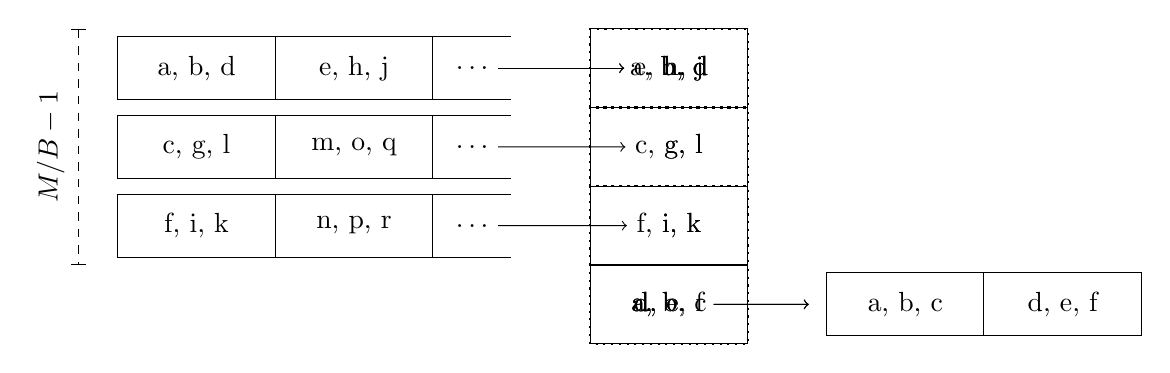
\begin{tikzpicture}
      % Input Blocks
      \draw[] (0,0.1)  rectangle ++(2,0.8) node[pos=.5] {a, b, d};
      \draw[] (2,0.1)  rectangle ++(2,0.8) node[pos=.5] {e, h, j};
      \draw[-] (4,0.9) -- ++(1,0);
      \node[] at (4.5,0.5) (i1) {$\dots$};
      \draw[-] (4,0.1) -- ++(1,0);

      \draw[] (0,-0.9) rectangle ++(2,0.8) node[pos=.5] {c, g, l};
      \draw[] (2,-0.9) rectangle ++(2,0.8) node[pos=.5] {m, o, q};
      \draw[-] (4,-0.1) -- ++(1,0);
      \node[] at (4.5,-0.5) (i2) {$\dots$};
      \draw[-] (4,-0.9) -- ++(1,0);

      \draw[] (0,-1.9) rectangle ++(2,0.8) node[pos=.5] (i3b1) {f, i, k};
      \draw[] (2,-1.9) rectangle ++(2,0.8) node[pos=.5] (i3b2) {n, p, r};
      \draw[-] (4,-1.1) -- ++(1,0);
      \node[] at (4.5,-1.5) (i3) {$\dots$};
      \draw[-] (4,-1.9) -- ++(1,0);

      % Input Blocks Size
      \draw [black, dashed, |-|] (-0.5,1) -- node[pos=.5, rotate=90, yshift=10] {$M/B-1$} (-0.5,-2);

      % Memory

      % - I1
      \draw[dotted, thick] (6,0)  rectangle ++(2,1) node[pos=.5] (M1) {};

      \onslide<2-3> {
        \draw[] (6,0)  rectangle ++(2,1) node[pos=.5] (M1) {a, b, d};
      }
      \onslide<4> {
        \draw[] (6,0)  rectangle ++(2,1) node[pos=.5] (M1) {\phantom{a, }b, d};
      }
      \onslide<5-8> {
        \draw[] (6,0)  rectangle ++(2,1) node[pos=.5] (M1) {\phantom{a, b, }d};
      }

      \onslide<10-11> {
        \draw[] (6,0)  rectangle ++(2,1) node[pos=.5] (M1) {e, h, j};
      }
      \onslide<12-> {
        \draw[] (6,0)  rectangle ++(2,1) node[pos=.5] (M1) {\phantom{e, }h, j};
      }

      % - I2
      \draw[dotted, thick] (6,-1)  rectangle ++(2,1) node[pos=.5] (M2) {};

      \onslide<2-5>{
        \draw[] (6,-1)  rectangle ++(2,1) node[pos=.5] (M2) {c, g, l};
      }
      \onslide<6->{
        \draw[] (6,-1)  rectangle ++(2,1) node[pos=.5] (M2) {\phantom{c, }g, l};
      }

      % - I3
      \draw[dotted, thick] (6,-2)  rectangle ++(2,1) node[pos=.5] (M3) {};

      \onslide<2-12>{
        \draw[] (6,-2)  rectangle ++(2,1) node[pos=.5] (M3) {f, i, k};
      }
      \onslide<13->{
        \draw[] (6,-2)  rectangle ++(2,1) node[pos=.5] (M3) {\phantom{f, }i, k};
      }

      % - O
      \draw[dotted, thick] (6,-3)  rectangle ++(2,1) node[pos=.5] (M4) {};

      \onslide<4> {
        \draw[] (6,-3)  rectangle ++(2,1) node[pos=.5] (M4) {a\phantom{, b, c}};
      }
      \onslide<5> {
        \draw[] (6,-3)  rectangle ++(2,1) node[pos=.5] (M4) {a, b\phantom{, c}};
      }
      \onslide<6> {
        \draw[] (6,-3)  rectangle ++(2,1) node[pos=.5] (M4) {a, b, c};
      }

      \onslide<9-11> {
        \draw[] (6,-3)  rectangle ++(2,1) node[pos=.5] (M4) {d\phantom{, e, f}};
      }
      \onslide<12> {
        \draw[] (6,-3)  rectangle ++(2,1) node[pos=.5] (M4) {d, e\phantom{, f}};
      }
      \onslide<13> {
        \draw[] (6,-3)  rectangle ++(2,1) node[pos=.5] (M4) {d, e, f};
      }

      % Output blocks
      \node[] at (8.9,-2.5) (o) {};
      \onslide<7-> {
        \draw[] (9,-2.9)   rectangle ++(2,0.8) node[pos=.5] (ob1) {a, b, c};
      }
      \onslide<14-> {
        \draw[] (11,-2.9) rectangle ++(2,0.8) node[pos=.5] (ob2) {d, e, f};
      }

      % Arrows
      \onslide<2> {
        \draw[->]
          (i1) edge (M1)
          (i2) edge (M2)
          (i3) edge (M3)
        ;
      }
      \onslide<7> {
        \draw[->] (M4) edge (o);
      }
      \onslide<10> {
        \draw[->] (i1) edge (M1);
      }
      \onslide<14> {
        \draw[->] (M4) edge (o);
      }
    \end{tikzpicture}
  \end{figure}

\end{frame}

\begin{frame}
  \frametitle{I/O Model : M/B-way Mergesort\\Aggarwal and Vitter '87}

    \begin{figure}
    \centering

    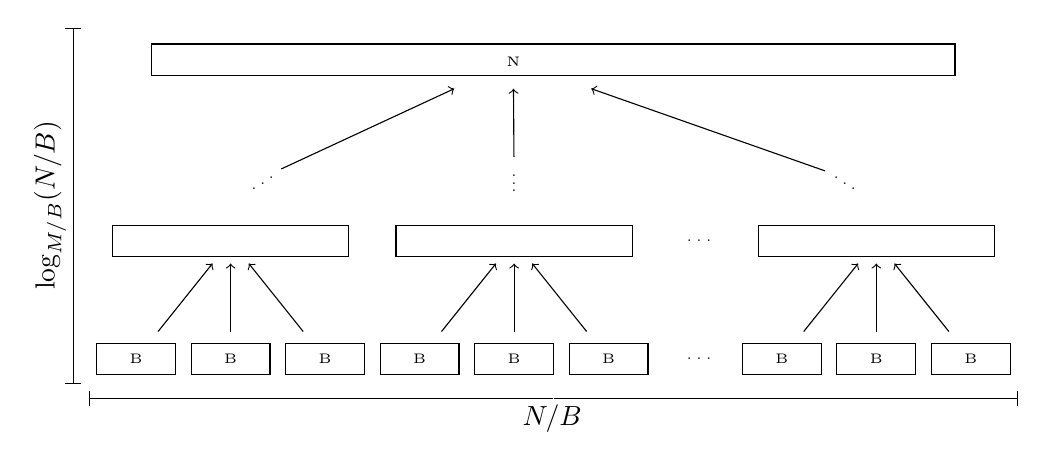
\begin{tikzpicture}
      % Base Case

      \tiny

      \onslide<2-> {
        \draw[] (0.0,0.0)  rectangle ++(1,0.4) node[pos=.5, inner sep=8] (l1b1) {B};
      }
      \onslide<3-> {
        \draw[] (1.2,0.0)  rectangle ++(1,0.4) node[pos=.5, inner sep=8] (l1b2) {B};
      }
      \onslide<4-> {
        \draw[] (2.4,0.0)  rectangle ++(1,0.4) node[pos=.5, inner sep=8] (l1b3) {B};
      }
      \onslide<5-> {
        \draw[] (3.6,0.0)  rectangle ++(1,0.4) node[pos=.5, inner sep=8] (l1b4) {B};
      }
      \onslide<6-> {
        \draw[] (4.8,0.0)  rectangle ++(1,0.4) node[pos=.5, inner sep=8] (l1b5) {B};
      }
      \onslide<7-> {
        \draw[] (6.0,0.0)  rectangle ++(1,0.4) node[pos=.5, inner sep=8] (l1b6) {B};
      }
      \onslide<8-> {
        \node at (7.65,0.2) {$\dots$};
        \draw[] (8.2,0.0)  rectangle ++(1,0.4) node[pos=.5, inner sep=8] (l1b7) {B};
      }
      \onslide<9-> {
        \draw[] (9.4,0.0)  rectangle ++(1,0.4) node[pos=.5, inner sep=8] (l1b8) {B};
      }
      \onslide<10-> {
        \draw[] (10.6,0.0) rectangle ++(1,0.4) node[pos=.5, inner sep=8] (l1b9) {B};

        % HACK: For some reason, when doing this horisontally, we get an
        %       unwanted horizontal '|' at the beginning.
        \draw[-|] (5.7,-0.3) edge ++(-5.8,0.0);
        \draw[-|] (5.9,-0.3) edge node[pos=-0.-0.02, below] {\normalsize $N/B$} ++(5.8,0.0);
      }

      % Merge level

      \onslide<11-> {
        \draw[] (0.2,1.5) rectangle ++(3.0,0.4) node[pos=.5, inner sep=8] (l2b1) {};
        \draw[->]
          (l1b1) edge (l2b1)
          (l1b2) edge (l2b1)
          (l1b3) edge (l2b1)
        ;
      }

      \onslide<12-> {
        \draw[] (3.8,1.5) rectangle ++(3.0,0.4) node[pos=.5, inner sep=8] (l2b2) {};
        \draw[->]
          (l1b4) edge (l2b2)
          (l1b5) edge (l2b2)
          (l1b6) edge (l2b2)
        ;
      }

      \onslide<13-> {
        \node at (7.65,1.7) {$\dots$};

        \draw[] (8.4,1.5) rectangle ++(3.0,0.4) node[pos=.5, inner sep=8] (l2b3) {};
        \draw[->]
          (l1b7) edge (l2b3)
          (l1b8) edge (l2b3)
          (l1b9) edge (l2b3)
        ;
      }

      % Final Result
      \onslide<14-> {
        \node at (2.1,2.5) (dots1) {$\iddots$};
        \node at (5.3,2.5) (dots2) {$\vdots$};
        \node at (9.5,2.5) (dots3) {$\ddots$};

        \draw[] (0.7,3.8) rectangle ++(10.2,0.4) node[pos=.45, inner sep=8] (N)
          {\phantom{PHANTOM}N\phantom{PHANTOM}};

        \draw[->]
          (dots1) edge (N)
          (dots2) edge (N)
          (dots3) edge (N)
        ;
      }

      \onslide<15-> {
        % HACK: Again, we get the horizontal '|' at the beginning of the edge.
        \draw[-|] (-0.3,-0.1) edge
                    node[pos=0.5, left, rotate=90, above=] {\normalsize$\log_{M/B}(N/B)$}
                    ++(0,4.5)
                  ;
      }

    \end{tikzpicture}
  \end{figure}

\end{frame}

\begin{frame}
  \frametitle{I/O Model : M/B-way Mergesort\\Aggarwal and Vitter '87}

  { \Large%
    \begin{theorem}
      $N$ elements can be sorted in $\Theta(N/B \cdot \log_{M/B}(N/B))$ I/Os.
    \end{theorem}
  }
\end{frame}

\section{Graham Scan}

\blankframe

\begin{frame}
  \frametitle{Convex Hull : Graham Scan\\Graham '72}

  \textbf{Convex Hull}

  Compute the \emph{convex hull} for $N$ points in the plane.

  \begin{figure}
    \centering

    \begin{tikzpicture}[scale=1.6]
      \draw[fill] (0.0,  0.0) circle [radius=0.06] node (p0) {};
\draw[fill] (0.6,  0.4) circle [radius=0.06] node (p1) {};
\draw[fill] (1.2,  0.6) circle [radius=0.06] node (p2) {};
\draw[fill] (1.6,  0.5) circle [radius=0.06] node (p3) {};
\draw[fill] (1.9,  0.1) circle [radius=0.06] node (p4) {};
\draw[fill] (2.2, -0.8) circle [radius=0.06] node (p5) {};
\draw[fill] (2.7, -0.1) circle [radius=0.06] node (p6) {};
\draw[fill] (3.3,  0.1) circle [radius=0.06] node (p7) {};

    \end{tikzpicture}
  \end{figure}

  \begin{theorem}
    Convex Hull can be computed in $O(N/B \cdot \log_{M/B}(N/B))$ I/Os.
  \end{theorem}
\end{frame}

\begin{frame}
  \frametitle{Convex Hull : Graham Scan\\Graham '72}

  \begin{columns}
    \begin{column}{0.6\linewidth}
      Upper Hull:
      \begin{itemize}
        \onslide<2-> {
        \item Sort input points by $x$-axis
        }
        \onslide<3-> {
        \item Initialize stack $S = [p_0, p_1]$
        }
        \onslide<4-> {
        \item For remaining points $p_i \in p_2, p_3, \dots, p_{N-1}$:
          \begin{enumerate}
          \item\label{graham scan: let}
            Let $p_s$, $p_t$ be the two top-most points of $S$

          \item While $p_s - p_t - p_i$ is a ``left-turn'':
            \begin{itemize}
            \item Pop $p_t$ and go-to \ref{graham scan: let}
            \end{itemize}

          \item Push $p_i$ onto $S$
          \end{enumerate}
        }
      \end{itemize}

      \onslide<13-> {
        Lower Hull:
        \begin{itemize}
        \item Symmetric...
        \end{itemize}
      }
    \end{column}
    \begin{column}{0.4\linewidth}
      \begin{figure}
        \centering
        \begin{tikzpicture}[scale=1.4]
          \draw[fill] (0.0,  0.0) circle [radius=0.06] node (p0) {};
\draw[fill] (0.6,  0.4) circle [radius=0.06] node (p1) {};
\draw[fill] (1.2,  0.6) circle [radius=0.06] node (p2) {};
\draw[fill] (1.6,  0.5) circle [radius=0.06] node (p3) {};
\draw[fill] (1.9,  0.1) circle [radius=0.06] node (p4) {};
\draw[fill] (2.2, -0.8) circle [radius=0.06] node (p5) {};
\draw[fill] (2.7, -0.1) circle [radius=0.06] node (p6) {};
\draw[fill] (3.3,  0.1) circle [radius=0.06] node (p7) {};

          \onslide<13-> {
            \draw[very thick, densely dotted]
              (p7) edge (p5)
              (p5) edge (p0)
            ;
          }

          \onslide<2-> {
            \node[black, below=0 of p0] (p0text) {$p_0$};
\node[black, above=0 of p1] (p1text) {$p_1$};
\node[black, above=0 of p2] (p2text) {$p_2$};
\node[black, above right=-0.1 and -0.1 of p3] (p3text) {$p_3$};
\node[black, below left=-0.1 and -0.1 of p4] (p4text) {$p_4$};
\node[black, below=0 of p5] (p5text) {$p_5$};
\node[black, below left=-0.1 and -0.1 of p6] (p6text) {$p_6$};
\node[black, below=0 of p7] (p7text) {$p_7$};

          }

          % edges
          \onslide<3->  { \draw[very thick, densely dotted] (p0) edge (p1); }
          \onslide<4->  { \draw[very thick, densely dotted] (p1) edge (p2); }
          \onslide<5->  { \draw[very thick, densely dotted] (p2) edge (p3); }
          \onslide<6-8> { \draw[very thick, densely dotted] (p3) edge (p4); }
          \onslide<7>   { \draw[very thick, densely dotted] (p4) edge (p5); }
          \onslide<10>  { \draw[very thick, densely dotted] (p3) edge (p6); }
          \onslide<12-> { \draw[very thick, densely dotted] (p3) edge (p7); }
        \end{tikzpicture}
      \end{figure}
    \end{column}
  \end{columns}
\end{frame}

\section{Trees & Priority Queues}

\blankframe

\begin{frame}
  \frametitle{\only<1>{a--b}\only<2->{Buffer} Tree \\%
    \only<1>{Huddleston and Mehlhorn '82}%
    \only<2->{Arge '95}%
  }

  \begin{figure}
    \centering

    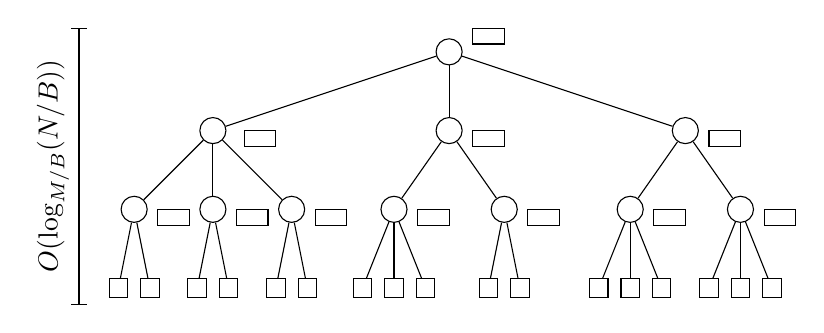
\begin{tikzpicture}
            % Root Level
      \node[draw = black, shape = circle] at (0,0)
      (r) {};

      % Children level 1
      \node[draw = black, shape = circle] at (-3,-1)
      (l1c1) {};

      \node[draw = black, shape = circle] at (0,-1)
      (l1c2) {};

      \node[draw = black, shape = circle] at (3,-1)
      (l1c3) {};

      % Children level 2
      \node[draw = black, shape = circle] at (-4,-2)
      (l2c1) {};
      \node[draw = black, shape = circle] at (-3,-2)
      (l2c2) {};
      \node[draw = black, shape = circle] at (-2,-2)
      (l2c3) {};

      \node[draw = black, shape = circle] at (-0.7,-2)
      (l2c4) {};
      \node[draw = black, shape = circle] at (0.7,-2)
      (l2c5) {};

      \node[draw = black, shape = circle] at (2.3,-2)
      (l2c6) {};
      \node[draw = black, shape = circle] at (3.7,-2)
      (l2c7) {};

      % Leaf level
      \node[draw = black, shape = rectangle] at (-4.2,-3)
      (l3c1) {};
      \node[draw = black, shape = rectangle] at (-3.8,-3)
      (l3c2) {};

      \node[draw = black, shape = rectangle] at (-3.2,-3)
      (l3c3) {};
      \node[draw = black, shape = rectangle] at (-2.8,-3)
      (l3c4) {};

      \node[draw = black, shape = rectangle] at (-2.2,-3)
      (l3c5) {};
      \node[draw = black, shape = rectangle] at (-1.8,-3)
      (l3c6) {};

      \node[draw = black, shape = rectangle] at (-1.1,-3)
      (l3c7) {};
      \node[draw = black, shape = rectangle] at (-0.7,-3)
      (l3c8) {};
      \node[draw = black, shape = rectangle] at (-0.3,-3)
      (l3c9) {};

      \node[draw = black, shape = rectangle] at (0.5,-3)
      (l3c10) {};
      \node[draw = black, shape = rectangle] at (0.9,-3)
      (l3c11) {};

      \node[draw = black, shape = rectangle] at (1.9,-3)
      (l3c12) {};
      \node[draw = black, shape = rectangle] at (2.3,-3)
      (l3c13) {};
      \node[draw = black, shape = rectangle] at (2.7,-3)
      (l3c14) {};

      \node[draw = black, shape = rectangle] at (3.3,-3)
      (l3c15) {};
      \node[draw = black, shape = rectangle] at (3.7,-3)
      (l3c16) {};
      \node[draw = black, shape = rectangle] at (4.1,-3)
      (l3c17) {};

      % Edges
      \draw[-]
        % Root - L1
        (r) edge (l1c1) edge (l1c2) edge (l1c3)
        % L1 - L2
        (l1c1) edge (l2c1) edge (l2c2) edge (l2c3)
        (l1c2) edge (l2c4) edge (l2c5)
        (l1c3) edge (l2c6) edge (l2c7)
        % L2 - L3
        (l2c1) edge (l3c1) edge (l3c2)
        (l2c2) edge (l3c3) edge (l3c4)
        (l2c3) edge (l3c5) edge (l3c6)
        (l2c4) edge (l3c7) edge (l3c8) edge (l3c9)
        (l2c5) edge (l3c10) edge (l3c11)
        (l2c6) edge (l3c12) edge (l3c13) edge (l3c14)
        (l2c7) edge (l3c15) edge (l3c16) edge (l3c17)
      ;


      % Vertical
      \onslide<2-> {
        \draw[-|] (-4.7,-3.2) edge
          node[pos=0.5, left, rotate=90, above=] {$O(\log_{M/B}(N/B))$}
          ++(0,3.5)
        ;
      }

      % Buffers
      \onslide<3-> {
        \draw[] (0.3,0.1) rectangle ++(0.4,0.2);

        \draw[] (-2.6,-1.2) rectangle ++(0.4,0.2);
        \draw[] ( 0.3,-1.2) rectangle ++(0.4,0.2);
        \draw[] ( 3.3,-1.2) rectangle ++(0.4,0.2);

        \draw[] (-3.7,-2.2) rectangle ++(0.4,0.2);
        \draw[] (-2.7,-2.2) rectangle ++(0.4,0.2);
        \draw[] (-1.7,-2.2) rectangle ++(0.4,0.2);

        \draw[] (-0.4,-2.2) rectangle ++(0.4,0.2);
        \draw[] ( 1.0,-2.2) rectangle ++(0.4,0.2);

        \draw[] ( 2.6,-2.2) rectangle ++(0.4,0.2);
        \draw[] ( 4.0,-2.2) rectangle ++(0.4,0.2);
      }
    \end{tikzpicture}
  \end{figure}

  \onslide<2-> {
    \begin{equation*}
      \qquad a = \frac{1}{4} M/B , \qquad b = M/B, \qquad \text{Leaf Size} = B
    \end{equation*}
  }
\end{frame}

\begin{frame}
  \frametitle{Buffer Tree \\ Arge '95}

  
  \begin{figure}
    \centering

    \begin{tikzpicture}
      % Root
      \node[draw = black, shape = circle] at (0,0)
      (r) {$0;42$};

      \draw[] (0.7,0.1) rectangle ++(5.8,0.8);
      \onslide<2> {
        \draw[] (0.7,0.1) rectangle ++(5.8,0.8) node[pos=0.5]
        {\texttt{ins(21)}\phantom{, \texttt{ins(64)}, \texttt{del(21)}, ...}};
      }
      \onslide<3> {
        \draw[] (0.7,0.1) rectangle ++(5.8,0.8) node[pos=0.5]
        {\texttt{ins(21)}, \texttt{ins(64)}\phantom{, \texttt{del(21)}, ...}};
      }
      \onslide<4> {
        \draw[] (0.7,0.1) rectangle ++(5.8,0.8) node[pos=0.5]
        {\texttt{ins(21)}, \texttt{ins(64)}, \texttt{del(21)}\phantom{, ...}};
      }
      \onslide<5> {
        \draw[] (0.7,0.1) rectangle ++(5.8,0.8) node[pos=0.5]
        {\texttt{ins(21)}, \texttt{ins(64)}, \texttt{del(21)}, ...};
      }
      \onslide<5-> {
        % HACK: For some reason, when doing this horisontally, we get an
        % unwanted horizontal '|' at the beginning.
        \draw[-|] (3.5,1.3) edge ++(-2.9,0.0);
        \draw[-|] (3.7,1.3) edge node[pos=-0.-0.02, above] {$\tfrac{1}{2} M/B$+} ++(2.9,0.0);
      }
      \onslide<6> {
        \draw[] (0.7,0.1) rectangle ++(5.8,0.8) node[pos=0.5]
        {\texttt{ins(21)}, \texttt{del(21)}, \texttt{ins(64)}, ...};
      }
      \onslide<7> {
        \draw[] (0.7,0.1) rectangle ++(5.8,0.8) node[pos=0.5]
        {\sout{\texttt{ins(21)}}, \sout{\texttt{del(21)}}, \texttt{ins(64)}, ...};
      }
      \onslide<8> {
        \draw[] (0.7,0.1) rectangle ++(5.8,0.8) node[pos=0.5]
        {\sout{\texttt{ins(21)}}, \sout{\texttt{del(21)}}\phantom{, \texttt{ins(64)}, ...}};
      }

      % Left Child
      \node[draw = black, shape = circle] at (-4,-2)
      (c1) {\phantom{0;42}};

      \draw[] (-0.8,-3) -- ++(-2.5,0) -- ++(0,0.8) -- ++(2.5,0);
      \onslide<8-> { \node at (-2.6, -2.6) {...}; }

      % Middle Child
      \node[draw = black, shape = circle] at (0,-2)
      (c2) {\phantom{0;42}};

      \draw[] (3.2,-3) -- ++(-2.5,0) -- ++(0,0.8) -- ++(2.5,0);
      \onslide<8-> { \node at (1.4, -2.6) {...}; }

      % Right Child
      \node[draw = black, shape = circle] at (4,-2)
      (c3) {\phantom{0;42}};

      \draw[] (7.2,-3) -- ++(-2.5,0) -- ++(0,0.8) -- ++(2.5,0);
      % \onslide<-7> { \node at (5.4, -2.6) {...}; }
      \onslide<8-> { \node at (5.9, -2.6) {\texttt{ins(64)}, ...}; }

      % Edges
      \draw[-] (r) edge (c1) edge (c2) edge (c3);
    \end{tikzpicture}
  \end{figure}

\end{frame}

\begin{frame}
  \frametitle{Buffer Tree \\ Arge '95}

  \begin{theorem}
    A \emph{Buffer Tree} can resolve $N$ \texttt{insert}s and \texttt{delete}s
    in $\Theta(N/B \cdot \log_{M/B}(N/B))$ I/Os.
  \end{theorem}

  \pause
  \begin{theorem}
    A \emph{Buffer Tree} with $N$ requests can empty all its buffers, and output
    all remaining sorted elements, in $\Theta(N/B)$ I/Os.
  \end{theorem}

  \pause
  \vspace{10pt}

  \begin{corollary}
    An I/O-efficient \emph{Priority Queue} can resolve $N$ \texttt{push} and
    \texttt{deletemin} operations in $\Theta(N/B \cdot \log_{M/B}(N/B))$ I/Os.
  \end{corollary}
  \begin{proof}
    \small

    Use an $M/2$ sized internal memory priority queue, \texttt{pq}. If
    \texttt{pq} overflows, move $M/4$ the largest elements to a Buffer Tree,
    \texttt{t}. If \texttt{pq} underflows, obtain the $M/4$ smallest elements
    from \texttt{t}.
  \end{proof}
\end{frame}

\section{Time-forward Processing}

\blankframe

\begin{frame}
  \frametitle{Binary Decision Diagrams \\ Arge '96, S{\o}lvsten '22}

  \begin{columns}
    \begin{column}{0.5\linewidth}
      \textbf{\#Paths}

      Given a Binary Decision Diagram of $N$ nodes, compute the number of paths
      from the root to the $\top$ terminal.

      \vspace{20pt}
      \begin{theorem}
        \emph{\#Paths} can be computed in $O(N/B \cdot \log_{M/B}(N/B))$ I/Os.
      \end{theorem}

    \end{column}
    \begin{column}{0.5\linewidth}
      \begin{figure}
        \centering

        \begin{tikzpicture}[scale=0.8, every node/.style={transform shape}]
            % nodes
  \node[shape = circle, draw = black]
  (0) {$x_0$};

  \node[shape = circle, draw = black, below right= .4cm and .5cm of 0]
  (1) {$x_1$};

  \node[shape = circle, draw = black, below left=.4cm and .5cm of 1]
  (2) {$x_2$};

  \node[shape = circle, draw = black, below left=.4cm and .5cm of 2]
  (31) {$x_3$};
  \node[shape = circle, draw = black, below right=.4cm and .5cm of 2]
  (32) {$x_3$};

  % leafs
  \node[shape = rectangle, draw = black, below=.4cm of 31]
  (sink_T) {$\top$};

  \node[shape = rectangle, draw = black, below=.4cm of 32]
  (sink_F) {$\bot$};

  % arcs
  \draw[->, dashed]
    (0)  edge (2)
    (1)  edge (2)
    (2)  edge (31)
    (31) edge (sink_T)
    (32) edge (sink_F)
  ;

  \draw[->]
    (0)  edge (1)
    (1)  edge (32)
    (2)  edge (32)
    (31) edge (sink_F)
    (32) edge (sink_T)
  ;
        \end{tikzpicture}

        \caption{\small \textbf{(a)} $(x_0 \wedge x_1 \wedge x_3) \vee (x_2 \oplus x_3)$}
      \end{figure}
    \end{column}
  \end{columns}
\end{frame}


\begin{frame}
  \frametitle{Binary Decision Diagrams \\ Arge '96, S{\o}lvsten '22}

  \begin{figure}
    \centering

    \begin{subfigure}[b]{0.45\linewidth}
      \centering

      \begin{tikzpicture}[scale=1, every node/.style={transform shape}]
          % nodes
  \node[shape = circle, draw = black]
  (0) {$x_0$};

  \node[shape = circle, draw = black, below right= .4cm and .5cm of 0]
  (1) {$x_1$};

  \node[shape = circle, draw = black, below left=.4cm and .5cm of 1]
  (2) {$x_2$};

  \node[shape = circle, draw = black, below left=.4cm and .5cm of 2]
  (31) {$x_3$};
  \node[shape = circle, draw = black, below right=.4cm and .5cm of 2]
  (32) {$x_3$};

  % leafs
  \node[shape = rectangle, draw = black, below=.4cm of 31]
  (sink_T) {$\top$};

  \node[shape = rectangle, draw = black, below=.4cm of 32]
  (sink_F) {$\bot$};

  % arcs
  \draw[->, dashed]
    (0)  edge (2)
    (1)  edge (2)
    (2)  edge (31)
    (31) edge (sink_T)
    (32) edge (sink_F)
  ;

  \draw[->]
    (0)  edge (1)
    (1)  edge (32)
    (2)  edge (32)
    (31) edge (sink_F)
    (32) edge (sink_T)
  ;
      \end{tikzpicture}

      \emph{\small Decision Diagram}
    \end{subfigure}
    \hspace{20pt}
    \begin{subfigure}[b]{0.45\linewidth}
      \centering
      { \small
        \begin{tabular}{r c l}
          [ & $\triple{(0,0)}{(2,0)}{(1,0)}$ & ,
          \\ \\
            & $\triple{(1,0)}{(2,0)}{(3,1)}$ & ,
          \\ \\
            & $\triple{(2,0)}{(3,0)}{(3,1)}$ & ,
          \\ \\
            & $\triple{(3,0)}{\top}{\bot}$   & ,
          \\ \\
            & $\triple{(3,1)}{\bot}{\top}$   & ]
        \end{tabular}
        \vspace{6pt}
      }

      \emph{\small On-Disk Format}
    \end{subfigure}

    \caption{\textbf{(a)} $(x_0 \wedge x_1 \wedge x_3) \vee (x_2 \oplus x_3)$}
  \end{figure}

\end{frame}

\begin{frame}[t]
  \frametitle{Binary Decision Diagrams \\ Arge '96, S{\o}lvsten '22}

  % HACK: The slide below is only designed for single-line frametitles.
  \vspace{-18pt}

  \begin{figure}
    \centering

    \begin{tikzpicture}[scale=0.9, every node/.style={transform shape}]
      % nodes
\node[shape = circle, draw = black] (n) {\small $(i,\texttt{id})$};

\node[below left  = 1 and 1 of n]  (low) {$\alpha$};
\node[below right = 1 and 1 of n] (high) {$\beta$};

% parent dummies

\node[above left  = 0.5 and 1 of n]  (p1) {$n_1$};
\node[above       = 0.5 of n] (p2) {$n_2$};
\node[above right = 0.5 and 1 of n] (p3) {$n_3$};

% arcs
\draw[->, dashed] (n) edge node[above left]{$\sum_i n_i$} (low);
\draw[->]         (n) edge node[above right]{$\sum_i n_i$} (high);

\draw[->, dotted, thick]
(p1) edge[bend left] (n)
(p2) edge (n)
(p3) edge[bend right] (n)
;

    \end{tikzpicture}
  \end{figure}

  \only<1>{
    \begin{center}
      {\Large \textbf{Idea}}

      {\large Count the number of in-going paths to each node.}
    \end{center}
  }

  \only<2->{
    \begin{center}
      {\Large \textbf{Time-Forward Processing}}

      Defer work with $Q_{\mathit{count}}$ : \texttt{PriorityQueue}$\langle (\arc{s}{}{t}, \quad
      \N) \rangle$ sorted on $t$ in ascending order.

      $(\arc{(i,\texttt{id})}{\bot}{\alpha}, \quad \sum_i n_i)$, \qquad
      $(\arc{(i,\texttt{id})}{\top}{\beta}, \quad \sum_i n_i)$
    \end{center}
  }
\end{frame}

\begin{frame}
  \frametitle{Binary Decision Diagrams \\ Arge '96, S{\o}lvsten '22}

  \begin{columns}
  \begin{column}{0.49\textwidth}

    \begin{figure}
      \centering

      \begin{subfigure}{1\linewidth}
        \centering

        \begin{tikzpicture}[scale=0.9, every node/.style={transform shape}]
          % nodes
          \node[shape = circle, draw = black]
          (0) {\tiny $(0,0)$};

          \node[shape = circle, draw = black, below right= .3cm and .5cm of 0]
          (1) {\tiny $(1,0)$};

          \node[shape = circle, draw = black, below left=.3cm and .5cm of 1]
          (2) {\tiny $(2,0)$};

          \node[shape = circle, draw = black, below left=.3cm and .5cm of 2]
          (31) {\tiny $(3,0)$};
          \node[shape = circle, draw = black, below right=.3cm and .5cm of 2]
          (32) {\tiny $(3,1)$};

          % leafs
          \node[shape = rectangle, draw = black, below=.4cm of 31]
          (sink_T) {$\top$};

          \node[shape = rectangle, draw = black, below=.4cm of 32]
          (sink_F) {$\bot$};

          % arcs
          \draw[->,dashed]
          (0) edge (2)
          (1) edge (2)
          (2) edge (31)
          (31) edge (sink_T)
          (32) edge (sink_F)
          ;

          \draw[->]
          (0) edge (1)
          (1) edge (32)
          (2) edge (32)
          (31) edge (sink_F)
          (32) edge (sink_T)
          ;

          % animations
          \onslide<3-5>{ % 0
            \node[shape = circle, orange, draw = orange]
            {\tiny $(0,0)$};
            \draw[->,dashed,orange] (0) edge (2);
            \draw[->,orange] (0) edge (1);
          }

          \onslide<6-9>{ % 1
            \node[shape = circle, orange, draw = orange, below right= .3cm and .5cm of 0]
            {\tiny $(1,0)$};
            \draw[->,dashed,orange] (1) edge (2);
            \draw[->,orange] (1) edge (32);
          }

          \onslide<10-14>{ % 2
            \node[shape = circle, orange, draw = orange, below left=.3cm and .5cm of 1]
            {\tiny $(2,0)$};
            \draw[->,dashed,orange] (2) edge (31);
            \draw[->,orange] (2) edge (32);
          }

          \onslide<15-18>{ % 31
            \node[shape = circle, orange, draw = orange, below left=.3cm and .5cm of 2]
            {\tiny $(3,0)$};
            \draw[->,dashed,orange] (31) edge (sink_T);
            \draw[->,orange] (31) edge (sink_F);
          }

          \onslide<19-22>{ % 32
            \node[shape = circle, orange, draw = orange, below right=.3cm and .5cm of 2]
            {\tiny $(3,1)$};
            \draw[->,dashed,orange] (32) edge (sink_F);
            \draw[->,orange] (32) edge (sink_T);
          }
        \end{tikzpicture}

        \caption{\small $(x_0 \wedge x_1 \wedge x_3) \vee (x_2 \oplus x_3)$}
      \end{subfigure}

      %\caption{In-order traversal of BDD}
    \end{figure}

  \end{column}
  \begin{column}{0.49\textwidth}
    \centering

    \onslide<5->{ \small
      \begin{tabular}{c c c}
        \onslide<5-22>{\hspace{10pt}Seek\hspace{10pt}}
        \onslide<5-22>{& \hspace{10pt}Sum\hspace{10pt}}
        \onslide<5-23>{& \hspace{10pt}Result\hspace{10pt}}
        \\
        \textcolor{orange}{%
        \only<5-8>{$(1,0)$}%
        \only<9-13>{$(2,0)$}%
        \only<14-17>{$(3,0)$}%
        \only<18-22>{$(3,1)$}%
        }
        &
        % (1,0)
          \only<5-6>{$0$}%
          \only<7-8>{$1$}%
          % (2,0)
          \only<9-10>{$0$}%
          \only<11>{$1$}%
          \only<12-13>{$2$}%
          % (3,0)
          \only<14-15>{$0$}%
          \only<16-17>{$2$}%
          % (3,1)
          \only<18-19>{$0$}%
          \only<20>{$1$}%
          \only<21-22>{$3$}%
        &
          \only<1-16>{$0$}%
          \only<17-21>{$2$}%
          \only<22-23>{$5$}%
      \end{tabular}
    }

    \vspace{20pt}

    \onslide<2->{
      {\footnotesize Priority Queue: $Q_{\mathit{count}}$:

        \begin{tabular}{rll}
          [ & \onslide<4-6>{$(\arc{(0,0)}{\top}{(1,0)}, \quad 1)$  & ,}
          \\
            & \onslide<4-10>{$(\arc{(0,0)}{\bot}{(2,0)}, \quad 1)$  & ,}
          \\
            & \onslide<8-11>{$(\arc{(1,0)}{\bot}{(2,0)}, \quad 1)$  & ,}
          \\
            & \onslide<13-15>{$(\arc{(2,0)}{\bot}{(3,0)}, \quad 2)$  & ,}
          \\
            & \onslide<8-19>{$(\arc{(1,0)}{\top}{(3,1)}, \quad 1)$   & ,}
          \\
            & \onslide<13-20>{$(\arc{(2,0)}{\top}{(3,1)}, \quad 2)$ }  & ]
        \end{tabular}
      }
    }

  \end{column}
\end{columns}

\end{frame}

\begin{frame}[plain,noframenumbering]{} % \blankframe until reveal
  \pause

  \begin{center}
    \vspace{8pt}

    {\Huge \textbf{Adiar}}

    \vspace{12pt}

    \textcolor{gray}{\small
      \href{http://github.com/ssoelvsten/adiar}{github.com/ssoelvsten/adiar}
    }
  \end{center}
\end{frame}

\begin{frame}
  \frametitle{Binary Decision Diagrams \\ Arge '96, S{\o}lvsten '22}

  \begin{figure}
    \centering
    \begin{subfigure}[b]{0.7\linewidth}
      \centering

      \begin{tikzpicture}
        \begin{axis}[%
          width=1\linewidth, height=0.55\linewidth,
          every tick label/.append style={font=\scriptsize},
          % x-axis
          xlabel={Instance Size (\# BDD nodes)},
          xmajorgrids=true,
          xmin=10000,
          xmax=1000000000000,
          xmode = log,
          % y-axis
          ymin=0.001,
          ymax=1000000,
          ymode=log,
          ytick={0.001,0.01,0.1,1,10,100,1000,10000,100000,1000000},
          ylabel={Time (s)},
          yminorgrids=false,
          ymajorgrids=true,
          grid style={dashed,black!20},
          ]

          \only<1-> {
            \addplot+ [style=plot_other]
            table {./data/queens_buddy_time.tex};

            \addplot+ [style=plot_other]
            table {./data/queens_cudd_time.tex};

            \addplot+ [style=plot_other]
            table {./data/queens_sylvan_time.tex};
          }

          \only<2-> {
            \addplot+ [style=plot_adiar]
            table {./data/queens_adiar_time.v1.2.0.tex};
          }
        \end{axis}

        \only<1-> {
          \node[color=black, rotate=90] at (5.85, 1.90) {\small $19.8$~GiB};
        }
        \only<2-> {
          \node[color=black, rotate=90] at (7.50, 2.75) {\small $736$~GiB};
        }
      \end{tikzpicture}
    \end{subfigure}
    \begin{subfigure}[b]{0.29\linewidth}
      \centering

      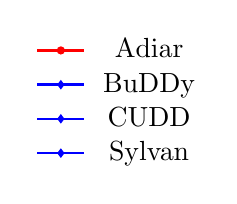
\begin{tikzpicture}
        \begin{customlegend}[
          legend columns=1,
          legend style={draw=none,column sep=1ex},
          legend entries={Adiar, BuDDy, CUDD, Sylvan}
          ]
          \addlegendimage{style=plot_adiar}
          \addlegendimage{style=plot_other}
          \addlegendimage{style=plot_other}
          \addlegendimage{style=plot_other}
        \end{customlegend}
      \end{tikzpicture}

      % HACK: Using [t] above does not do what I hoped it to.
      \vspace{50pt}
    \end{subfigure}
    \caption{Running time for the \emph{N-Queens} problems.}
  \end{figure}
\end{frame}

\blankframe

\section{References}

\begin{frame}[t]
  \frametitle{Further Reading :
    \only<1>{Foundations}%
    \only<2>{Data Structures}%
    \only<3>{Algorithms}%
    \only<4>{Libraries (C++)}
   }

  \large

  \only<1>{
    \begin{itemize}
    \item \textbf{Aggarwal and Vitter (1987)}

      \emph{``The Input/Output Complexity of Sorting and Related Problems''}

      {\color{gray}\normalsize The I/O-model, Sorting, Permutation, FFT, and
        Matrix transposition.}

    \item \textbf{Arge, Goodrich, Nelson, and Sitchinava (2008)}

      \emph{``Fundamental Parallel Algorithms for Private-cache Chip Multiprocessors.''}

      {\color{gray}\normalsize The I/O-model for Multi-Threading.}
    \end{itemize}
  }
  \only<2>{
    \begin{itemize}
    \item \textbf{Arge (1995)}

      \emph{``The Buffer Tree: A new technique for Optimal I/O-algorithms''}

      {\color{gray}\normalsize An I/O-efficient Tree, Priority Queue, and Range Tree.}

    \item \textbf{Sanders (2002)}

      \emph{``Fast Priority Queues for Cached Memory''}

      {\color{gray}\normalsize A much faster I/O-efficient Priority Queue.}

    \item \textbf{Agarwal, Arge and Yi (2006)}

      \emph{``I/O-Efficient Batched Union-Find and Its Applications to Terrain Analysis''}

      {\color{gray}\normalsize An I/O-efficient (Lazy) Union-Find.}
    \end{itemize}
  }
  \only<3>{
    \begin{itemize}
    \item \textbf{Goodrich, Tsay, Vengroff, and Vitter (1993)}

      \emph{``External-Memory Computational Geometry''}

      {\color{gray}\normalsize Distribution Sweeping and other algorithms.}

    \item \textbf{Chiang, Goodrich, Grove, Tamassia, Vengroff, and Vitter (1995)}

      \emph{``External-memory Graph Algorithms''}

      {\color{gray}\normalsize Time-forward Processing and other algorithms.}

    \item \textbf{Arge, Toma, Vitter (2001)}

      \emph{``I/O-Efficient Algorithms for Problems on Grid-Based Terrains''}

      {\color{gray}\normalsize The T{\footnotesize ERRA}F{\footnotesize LOW} algorithm.}
    \end{itemize}
  }
  \only<4>{
    \begin{itemize}
    \item \textbf{TPIE : Templated Portable I/O Environment}

      \href{https://github.com/thomasmoelhave/tpie}{\texttt{github.com/thomasmoelhave/tpie}}

      {\color{gray}\normalsize Duke University and Aarhus University}

    \item \textbf{STXXL : Standard Template library for XXL data sets}

      \href{https://github.com/stxxl/stxxl}{\texttt{github.com/stxxl/stxxl}}

      {\color{gray}\normalsize University of Karlsruhe}
    \end{itemize}
  }
\end{frame}

\begin{frame}[plain,noframenumbering]
  {\Large \textbf{Steffan Christ Sølvsten}}
  \vspace{1pt} {\hrule width0.45\linewidth}

  \vspace{5pt}

  \begin{itemize}
  \item[\faIcon{envelope}] \mailto{soelvsten@cs.au.dk}
  \item[\faIcon{twitter}] \href{https://www.twitter.com/ssoelvsten}{@ssoelvsten}
  \end{itemize}

  \vspace{10pt}

  {\Large \textbf{Adiar}}
  \vspace{1pt} {\hrule width0.45\linewidth}

  \vspace{5pt}

  \begin{itemize}
  \item[\faIcon{code}]
    \href{http://github.com/ssoelvsten/adiar}{github.com/ssoelvsten/adiar}
  \item[\faIcon{book}\hspace{2pt}]
    \href{http://ssoelvsten.github.io/adiar}{ssoelvsten.github.io/adiar}
  \end{itemize}


  \vspace{10pt}

  
\includegraphics[width=0.2\linewidth]{external/aulogo_uk_var2_black.eps}
\end{frame}

\blankframe

\section{Appendix}

\subsection{Distribution Sweeping}

\begin{frame}
  \frametitle{Distribution Sweeping\\Goodrich, Tsay, Vengroff, and Vitter '93}

  \textbf{Batched Range Searching}

  Given $N$ axis-parallel rectangles and $N$ points in the plane, compute for
  each point $p$ all rectangles containing $p$.

  \begin{figure}
    \centering
    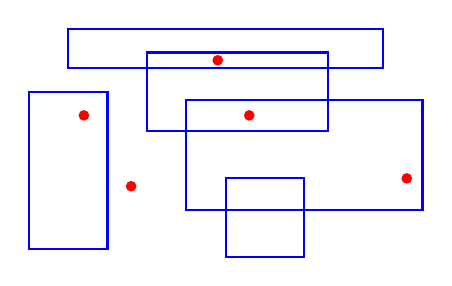
\begin{tikzpicture}
      % Rectangles
\draw[blue, thick] (0,0) rectangle ++(1,2);
\draw[blue, thick] (1.5,1.5) rectangle ++(2.3,1);
\draw[blue, thick] (2,0.5) rectangle ++(3,1.4);
\draw[blue, thick] (2.5,-0.1) rectangle ++(1,1);
\draw[blue, thick] (0.5,2.3) rectangle ++(4,0.5);

% Points
\draw [red, fill] (0.7, 1.7) circle [radius=0.06];
\draw [red, fill] (1.3, 0.8) circle [radius=0.06];
\draw [red, fill] (2.4, 2.4) circle [radius=0.06];
\draw [red, fill] (2.8, 1.7) circle [radius=0.06];
\draw [red, fill] (4.8, 0.9) circle [radius=0.06];

    \end{tikzpicture}
  \end{figure}

  \begin{theorem}
    Batched Range Searching can be solved in $O(\sort(N) + \scan(T))$ I/Os.
  \end{theorem}
\end{frame}

\begin{frame}
  \frametitle{Distribution Sweeping\\Goodrich, Tsay, Vengroff, and Vitter '93}

  \begin{columns}
    \begin{column}{0.6\linewidth}
      Preprocessing:
      \begin{itemize}
        \onslide<2->{
        \item Split each rectangle into two vertical
          lines.
        }

        \onslide<3->{
        \item Sort all lines and points by their $x$-value.
        }
      \end{itemize}
      Algorithm:
      \begin{itemize}
        \onslide<4->{
        \item Split all data into $\Theta(\sqrt{M/B})$ \emph{slabs}. Solve these
          recursively; output is given sorted by $y$-value.
        }

        \onslide<5->{
        \item Merge slabs together, report points between line segments outside
          its slab.
          \begin{itemize}
          \item Use $\Theta(\sqrt{M/B}^2) = \Theta(\sqrt{M/B})$ multi-slabs to
            maintain each \emph{active} rectangle.
          \item Output points and un-matched line segments.
          \end{itemize}
        }
      \end{itemize}
    \end{column}
    \begin{column}{0.4\linewidth}
      \begin{figure}
        \centering
        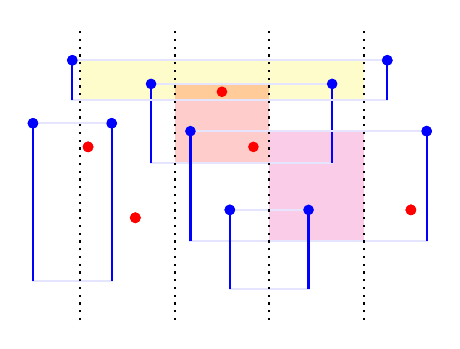
\begin{tikzpicture}
          \onslide<1>{
            % Rectangles
\draw[blue, thick] (0,0) rectangle ++(1,2);
\draw[blue, thick] (1.5,1.5) rectangle ++(2.3,1);
\draw[blue, thick] (2,0.5) rectangle ++(3,1.4);
\draw[blue, thick] (2.5,-0.1) rectangle ++(1,1);
\draw[blue, thick] (0.5,2.3) rectangle ++(4,0.5);

% Points
\draw [red, fill] (0.7, 1.7) circle [radius=0.06];
\draw [red, fill] (1.3, 0.8) circle [radius=0.06];
\draw [red, fill] (2.4, 2.4) circle [radius=0.06];
\draw [red, fill] (2.8, 1.7) circle [radius=0.06];
\draw [red, fill] (4.8, 0.9) circle [radius=0.06];

          }
          \onslide<2-3>{
            % Rectangles
\draw[blue!10!white, thick] (0,0) rectangle ++(1,2);
\draw[blue, thick] (0,0) -- (0,2) (1,0) -- (1,2);
\draw [blue, fill] (0,2) circle [radius=0.06];
\draw [blue, fill] (1,2) circle [radius=0.06];

\draw[blue!10!white, thick] (1.5,1.5) rectangle ++(2.3,1);
\draw[blue, thick] (1.5,1.5) -- (1.5,2.5) (3.8,1.5) -- (3.8,2.5);
\draw [blue, fill] (1.5,2.5) circle [radius=0.06];
\draw [blue, fill] (3.8,2.5) circle [radius=0.06];

\draw[blue!10!white, thick] (2,0.5) rectangle ++(3,1.4);
\draw[blue, thick] (2,0.5) -- (2,1.9) (5,0.5) -- (5,1.9);
\draw [blue, fill] (2,1.9) circle [radius=0.06];
\draw [blue, fill] (5,1.9) circle [radius=0.06];

\draw[blue!10!white, thick] (2.5,-0.1) rectangle ++(1,1);
\draw[blue, thick] (2.5,-0.1) -- (2.5,0.9) (3.5,-0.1) -- (3.5,0.9);
\draw [blue, fill] (2.5,0.9) circle [radius=0.06];
\draw [blue, fill] (3.5,0.9) circle [radius=0.06];

\draw[blue!10!white, thick] (0.5,2.3) rectangle ++(4,0.5);
\draw[blue, thick] (0.5,2.3) -- (0.5,2.8) (4.5,2.3) -- (4.5,2.8);
\draw [blue, fill] (0.5,2.8) circle [radius=0.06];
\draw [blue, fill] (4.5,2.8) circle [radius=0.06];

% Points
\draw [red, fill] (0.7, 1.7) circle [radius=0.06];
\draw [red, fill] (1.3, 0.8) circle [radius=0.06];
\draw [red, fill] (2.4, 2.4) circle [radius=0.06];
\draw [red, fill] (2.8, 1.7) circle [radius=0.06];
\draw [red, fill] (4.8, 0.9) circle [radius=0.06];

          }
          \onslide<5->{
            % Multi-slabs
\fill[yellow!20!white] (0.6,2.3) rectangle ++(3.6,0.5);
\fill[red!20!white] (1.8,1.5) rectangle ++(1.2,1);
\fill[orange!40!white] (1.8,2.3) rectangle ++(1.2,0.2);
\fill[magenta!20!white] (3,0.5) rectangle ++(1.2,1.4);
          }
          \onslide<4-5>{
            % Rectangles
% Rectangles
\draw[blue!10!white, thick] (0,0) rectangle ++(1,2);
\draw[blue, thick] (0,0) -- (0,2) (1,0) -- (1,2);
\draw [blue, fill] (0,2) circle [radius=0.06];
\draw [blue, fill] (1,2) circle [radius=0.06];

\draw[blue!10!white, thick] (1.5,1.5) rectangle ++(2.3,1);
\draw[blue, thick] (1.5,1.5) -- (1.5,2.5) (3.8,1.5) -- (3.8,2.5);
\draw [blue, fill] (1.5,2.5) circle [radius=0.06];
\draw [blue, fill] (3.8,2.5) circle [radius=0.06];

\draw[blue!10!white, thick] (2,0.5) rectangle ++(3,1.4);
\draw[blue, thick] (2,0.5) -- (2,1.9) (5,0.5) -- (5,1.9);
\draw [blue, fill] (2,1.9) circle [radius=0.06];
\draw [blue, fill] (5,1.9) circle [radius=0.06];

\draw[blue!10!white, thick] (2.5,-0.1) rectangle ++(1,1);
\draw[blue, thick] (2.5,-0.1) -- (2.5,0.9) (3.5,-0.1) -- (3.5,0.9);
\draw [blue, fill] (2.5,0.9) circle [radius=0.06];
\draw [blue, fill] (3.5,0.9) circle [radius=0.06];

\draw[blue!10!white, thick] (0.5,2.3) rectangle ++(4,0.5);
\draw[blue, thick] (0.5,2.3) -- (0.5,2.8) (4.5,2.3) -- (4.5,2.8);
\draw [blue, fill] (0.5,2.8) circle [radius=0.06];
\draw [blue, fill] (4.5,2.8) circle [radius=0.06];

% Points
\draw [red, fill] (0.7, 1.7) circle [radius=0.06];
\draw [red, fill] (1.3, 0.8) circle [radius=0.06];
\draw [red, fill] (2.4, 2.4) circle [radius=0.06];
\draw [red, fill] (2.8, 1.7) circle [radius=0.06];
\draw [red, fill] (4.8, 0.9) circle [radius=0.06];


% Slabs
\draw[black, thick, dotted]
  (0.6,-.5) -- ++(0,3.7)
  (1.8,-.5) -- ++(0,3.7)
  (3,-.5) -- ++(0,3.7)
  (4.2,-.5) -- ++(0,3.7)
;
          }
        \end{tikzpicture}

        \vspace{8pt}

        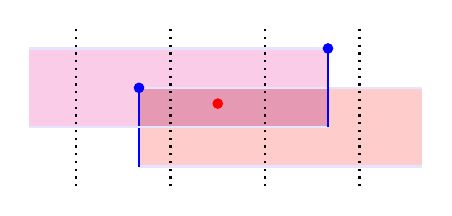
\begin{tikzpicture}
          \onslide<5>{
            % Multi-slabs
\fill[red!20!white] (1.4,0) rectangle ++(3.6,1);
\fill[magenta!20!white] (3.8,0.5) rectangle ++(-3.8,1);
\fill[purple!40!white] (1.4,0.5) rectangle ++(2.4,0.5);

% Rectangles
\draw[blue!10!white, thick] (1.4,0) -- (5,0) (1.4,1) -- (5,1);
\draw[blue, thick] (1.4,0) -- (1.4,1);
\draw [blue, fill] (1.4,1) circle [radius=0.06];

\draw[blue!10!white, thick] (3.8,0.5) -- (0,0.5) (3.8,1.5) -- (0,1.5);
\draw[blue, thick] (3.8,0.5) -- (3.8,1.5);
\draw [blue, fill] (3.8,1.5) circle [radius=0.06];

% Points
\draw [red, fill] (2.4, 0.8) circle [radius=0.06];

% Slabs
\draw[black, thick, dotted]
  (0.6,-0.25) -- ++(0,2)
  (1.8,-0.25) -- ++(0,2)
  (3,-0.25) -- ++(0,2)
  (4.2,-0.25) -- ++(0,2)
;

          }
        \end{tikzpicture}
      \end{figure}
    \end{column}
  \end{columns}
\end{frame}

\end{document}
